\documentclass{beamer}
%\setbeameroption{show notes on second screen=right} % Both
\setbeameroption{hide notes} % Only slides
%\setbeameroption{show only notes} % Only notes
% Theme choice:
\usetheme{Boadilla}
\usepackage{tikz}
\usepackage{tikz-feynman}
\usepackage{animate}
\usepackage{amsmath}
\usepackage{cancel}
\usepackage{multicol}
\usepackage{physics}
\usepackage{graphicx}
\usepackage{amsfonts}
\usepackage{caption}
\captionsetup{singlelinecheck=false}
\usefonttheme[onlymath]{serif}
%\usepackage{hyperref}
%\hypersetup{colorlinks = true,linkcolor = black,filecolor= black,urlcolor= black}
%\usepackage{subcaption}
\usepackage[backend=bibtex,bibencoding=utf8,doi=false,isbn=false,url=false,eprint=false,indexing=false,style=authortitle]{biblatex}
\addbibresource{library}
\AtEveryBibitem{%
	\clearname{translator}%
	\clearlist{publisher}%
	\clearfield{pagetotal}%
}
\usepackage{MnSymbol,wasysym}
\usepackage[toc,page]{appendix}
\usetikzlibrary{snakes}
\usetikzlibrary{shapes.geometric, calc}
\author[Presenter: VCD Phuong]{{\textit{Presenter}} \\
	Vo Chau Duc Phuong \inst{1} \\
	{\and} \\
	{\textit{Supervisors}} \\
	Dr. Huynh Thanh Duc \inst{2}}
\institute[HCMUS \& IAMI]{\inst{1} University of Science, Ho Chi Minh city\and %
	\inst{2} Institute of Applied Mechanics and Informatics}
% Title page details: 
\title[Linear Absorption Spectrum of $MoS_2$]{Calculation of the Linear-Absorption Spectrum of\\ an Ideal Two-Dimensional System of $\mathrm{MoS}_2$}
\begin{document}
\begin{frame}
		\titlepage
	\end{frame}
\begin{frame}{Table of Contents}
	\tableofcontents
\end{frame}
\section{Transition Metal Dichalcogenide Structure and Properties}
%\subsection{Structure}
\begin{frame}{Transition Metal Dichalcogenide Monolayer}
Transition metal dichalcogenide (TMD) is the compound has the form of MX$_2$.
\begin{center}
	\begin{figure}
		\label{elementtable}
\includegraphics[width = \linewidth]{images/MX2.png}
\caption{Transition metal dichalcogenide compound, $M$ is a transition metal atom and $X$ is a chalcogenides atoms}
	\end{figure}
\end{center}
	\end{frame}
\begin{frame}{Transition Metal Dichalcogenide Monolayer}
Some of the combination don't have the stable monolayer form. Others can be:
\begin{itemize}
	\item H (Honeycomb) structure (Example: MoS$_2$)
	\item T (centered honeycomb) structure (Example: NBS$_2$)
\end{itemize}
or both (Example: VS$_2$).\\
\quad These structure can affect the properties of the materials. TMD can be either metal (NbS$_2$, NbSe$_2$-T) or semiconductor (MoS$_2$)\footcite{ataca_stable_2012}.\\
\quad My thesis focused on MoS$_2$ monolayer (only have the H-structure), has the visible band gap in the band structure, which can be used in creating the transistor devices.\footcite{radisavljevic_single-layer_2011}
\end{frame}

\begin{frame}{Mono-layer structure}
\begin{multicols}{2}
	\begin{itemize}
\item The M (huge black dot) layer has been sandwiched by two \textcolor{green}{X} ( small green dot) layers as shown in top view (a) and side view (b).\\
\item They have the inverse asymmetry in real lattice.\\
\item The atomic lattice have the $D_{3h}$ symmetry group, result in the hexagon Brillouin Zone (BZ).
	\end{itemize}
	\columnbreak
	\vfill
	\begin{figure}
\label{Structure}
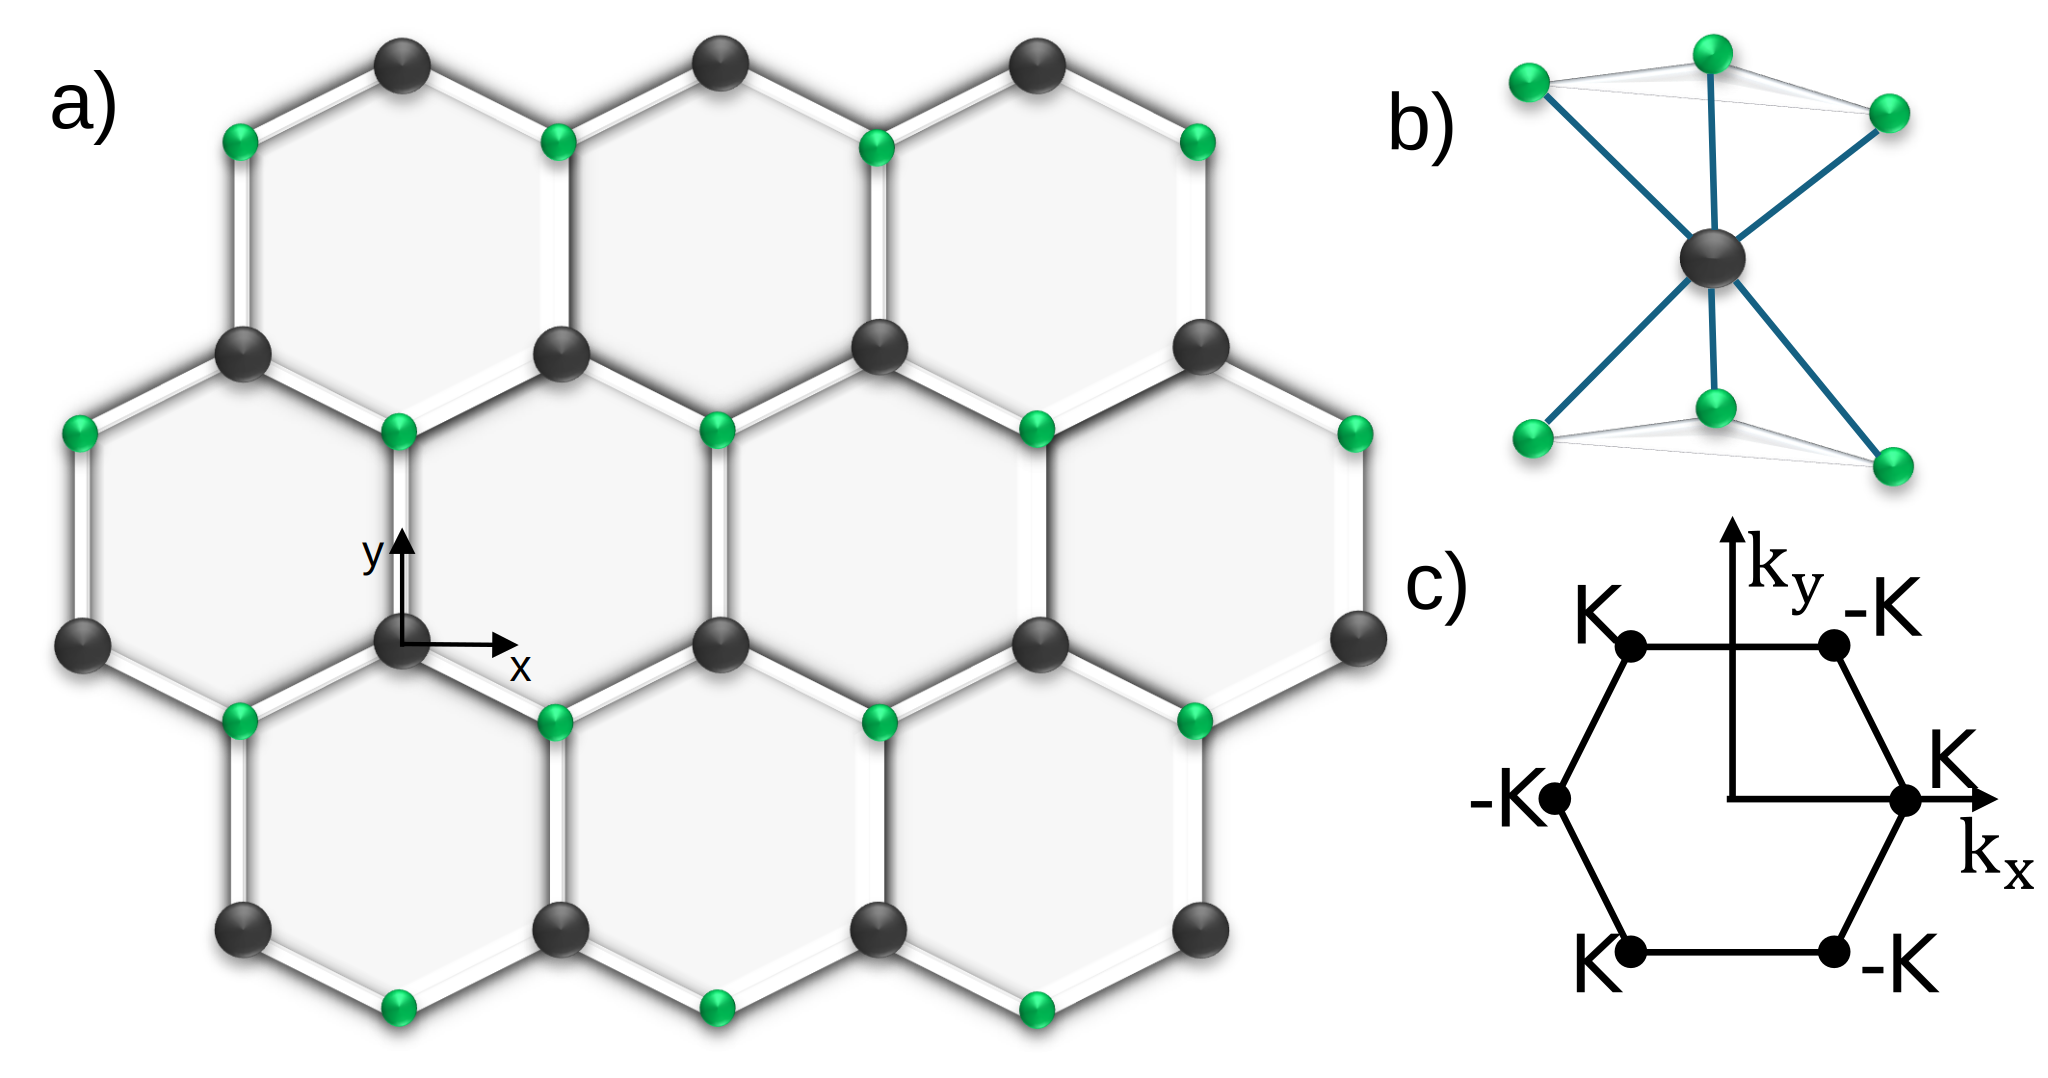
\includegraphics[width = \linewidth]{images/RS.pdf}
\caption{Structure and Brillouin Zone of Monolayer TMD, redrawing from\footcite{liu_three-band_2013}}
	\end{figure}
\end{multicols}
\end{frame}
%\subsection{Properties}
\begin{frame}{Splitting In The Band Structure}
\begin{multicols}{2}
\quad Huge split \textcolor{green}{$\Delta$} (hundreds of meV) in valley (K and -K points) of the band structure caused by the strong spin-orbit coupling (SOC) and the inversion asymmetry.\\
$\Rightarrow$ Applications in spintronic and optoelectronics\footcite{liu_electronic_2015}.
	\columnbreak
	\begin{center}
		\begin{figure}
			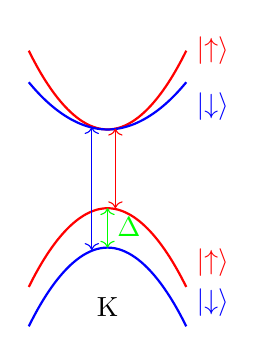
\begin{tikzpicture}
				\draw[red,thick] (0,1) parabola bend (1,0) (2,1)
				node[right] {$\ket{\uparrow}$};
				\draw[blue,thick] (0,0.6) parabola bend (1,0) (2,0.6) node[below right] {$\ket{\downarrow}$};
				%
				%
				\draw[red,thick] (0,-2) parabola bend (1,-1) (2,-2)
				node[above right] {$\ket{\uparrow}$};
				\draw[blue,thick] (0,-2.5) parabola bend (1,-1.5) (2,-2.5) node[above right] {$\ket{\downarrow}$};
				%
				%
				\draw[red, <->] (1.1,-1) to (1.1,0.01);
				\draw[blue, <->] (0.8,-1.53) to (0.8,0.03);
				\draw[green, <->] (1,-1.5) to (1,-1) node[below right] {$\Delta$};
				\node at (1,-2.5) [above] {K};
			\end{tikzpicture}
			\caption{The allowed optical  transition}
		\end{figure}
	\end{center}
\end{multicols}
\end{frame}
\section{Exciton}
\begin{frame}{Creation of An Exciton}
	\quad When an electron transit from valence band to a conduction band, it leave behind a hole.\\
	\quad This hole, acts like an positive charge, attract electrons to form a binding (called exciton).\\
	\vfill
\begin{figure}
	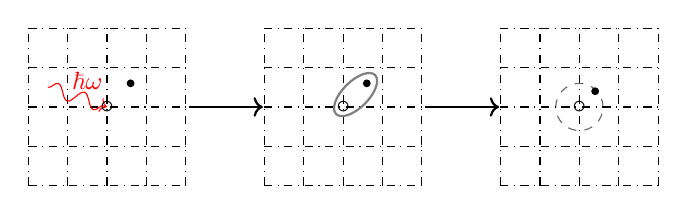
\begin{tikzpicture}
		\draw[step=5mm,black,thin,dash dot] (0,0) grid (2,2);
		\node at (1.3,1.3) [circle,fill,inner sep=1.pt] {};
		\draw[snake=snake,red,->] (0.25,1.25) node[above,xshift=0.5 cm, yshift=-0.15cm]{\small{$\hbar \omega$}} to (1,1);
		\node at (1.,1.) {$\circ$};
		%
		%
		\draw[->, black, thick] (2.04,1) to (2.98,1);
		%
		%
		\draw[step=5mm,black,thin,dash dot] (2.99,0) grid (5,2);
		\foreach \Point in {(4,1)}{
			\node at \Point {$\circ$};
		}
		\node at (4.3,1.3) [circle,fill,inner sep=1.pt] {};
		%
		%draw ellipse
		\node (p0) at (3.9,0.9) {};
		\node (qt) at (4.5,1.5) {};
		\path (p0.center) let \p1=($(qt.center)-(p0.center)$) in node[ellipse, minimum height=0.7cm, minimum width=0.1cm, anchor=south, thick, draw, gray, rotate={-atan2(\x1,\y1)}] {};
		%
		%
		
		\filldraw[color=black!60, fill=white!5, dashed](7,1) circle (0.3);
		\draw[->, black, thick] (5.04,1) to (5.98,1);
		\draw[step=5mm,black,thin,dash dot] (5.99,0) grid (8,2);
		\foreach \Point in {(7,1)}{
			\node at \Point {$\circ$};
		}
		\node at (7.2,1.2) [circle,fill,inner sep=1.pt] {};
		%
		%
	\end{tikzpicture}
	\caption{Illustration for the bouncing of the electron (black) and hole (circle)}
\end{figure}
\end{frame}
%next frame talk about the hydrogen-like exciton and binding energy.
\begin{frame}{Binding Energy of Exciton}
	\quad Interaction between a couple of electron and hole can be described as "a Hydrogen" atom, called "Exciton".\\
	\begin{equation}
 -\bigg[\frac{\hbar^2\nabla^2_{\textbf{r}}}{2m_r} + V(r)\bigg]\psi_{\nu}(\textbf{r}) = E_{\nu}(\textbf{r})\psi_{\nu}(\textbf{r}),
	\end{equation}
	\begin{multicols}{2}
where,\\
\begin{itemize}
	\item $V(r)$ is the Coulomb interaction with the form:
	\begin{equation}
	\label{Vr}
		V(r) = \frac{e^2}{\varepsilon |\textbf{r}|}
	\end{equation}
	\item $m_r = \frac{m_hm_e}{m_h +m_e}$ is the effective mass.
	\item $E_\nu (\textbf{r})$ is the binding energy of the exciton.
	\vfill
\end{itemize}
		\columnbreak
\begin{figure}
	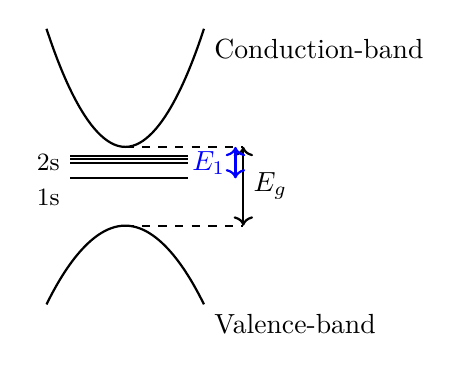
\begin{tikzpicture}
		\draw[black,thick] (0,1.5) parabola bend (1,0) (2,1.5)
		node[below right] {Conduction-band};
		%
		%
		\draw[black,thick] (0,-2) parabola bend (1,-1) (2,-2) node[below right] {Valence-band};
		\draw[black, thick] (0.3,-0.4) node[below left] {\small 1s} -- (1.8,-0.4) ;
		\draw[black, thick] (0.3,-0.15) -- (1.8,-0.15) node[right] {};
		\draw[black, thick] (0.3,-0.2) node[left] {\small 2s} -- (1.8,-0.2) ;
		\draw[black, thick] (0.3,-0.12) -- (1.8,-0.12) node[right] {};
		%
		%
		\draw[black, thick, <->] (2.5,0) to (2.5,-0.5) node[right] {$E_g$} to (2.5,-1);
		%\draw[red, thick, <->] (2.4,-0.4) to (2.4,-0.75) node[left] {$E_1$} to (2.4,-1);
		\draw[blue, thick, <->] (2.4,0) to (2.4,-0.2) node[left] {$E_1$} to (2.4,-0.4);
		\draw[black, thick, dashed] (1,0) -- (2.5,0);
		\draw[black, thick, dashed] (1,-1) -- (2.5,-1);
	\end{tikzpicture}
	\caption{Binding energy relative to the band gap}
\end{figure}
	\end{multicols}
\end{frame}
\begin{frame}{Exciton}
\quad The Coulomb interaction in the from of Eq. $(\ref{Vr})$ can only be valid if the bohr radius of "the Hydrogen-atom" around or smaller than the unit cell.\\
\quad In the bulk crystals with relative small dielectric constant, the exciton have the small binding energy.\\
Ex: GeAs\footcite{diakite2016accurateelectronictransportbulk}: $$E_b \approx 4.8 meV \ll E_g = 1.2-1.7 eV$$
\quad In these materials, the exciton binding energy can be neglected in simulations.
\end{frame}
\begin{frame}{Purpose}
\begin{center}
	So, why need to calculate it in TMD?
\end{center}
\begin{itemize}
\item In the 2-D materials (monolayer-TMD materials are in this), lack of system dimension causes decrease in the dielectric screening.
\item Large quantum confinement in nano-material (z-axis).
\end{itemize}
$\Rightarrow$ Increasing of exciton binding energy. Larger magnitude about two orders in compared with bulk semiconductor.\\
\begin{itemize}
\item Previous theories predict binding energy too large ($0.5-1$ \(eV\)), precisely experiment predicts significant smaller binding energy ($0.2-0.5$ \(eV\)).
\item Find a model not only simple but also precise enough for further research and application in industrial.
\end{itemize}
$\Rightarrow$ Look like enough for my bachelor's thesis \smiley{}.
\end{frame}
\section{Tight-binding Model}
\begin{frame}{Tight-binding Model}
\quad Start from the Hamiltonian for an independence electron:
\begin{equation}
	\label{H1e}
	H_{1e}(\textbf{r}) = -\frac{\hbar^2 \nabla^2}{2m} + \sum_{\text{i}} V(\textbf{r} - \textbf{R}_\text{i} -\textbf{r}_c),
\end{equation}
\quad where $\textbf{R}_i$ is the Bravais lattice position, $\textbf{r}_c$ is the relative position of atom inside unit cell. We neglected the motion of nucleus because in this case, the nucleus (Transistion metals and Chalcogenides) are very heavy in compare with the electron (Born-Oppenheimer approximation).\\\null\quad Assuming that the electron stay close to its atom and have little overlap on the neighboring sites. Therefore the wave function of each electron can be described by the linearly combination of atomic orbitals (LCAO).
\begin{equation}
	\label{key}
	\psi (\textbf{r}) = \sum_{n=1}^N \sum_{c = 1}^{N_c} \sum_{\alpha = 1}^{N_{orbital}} c_{\alpha c}(\textbf{R}_n) \phi_{\alpha}(\textbf{r}-\textbf{R}_n -\textbf{r}_c)
\end{equation}
$N, N_c, \text{and } N_{\alpha}$ is number of unit lattice of the system, number of atom in a basis and number of orbital of an atom, respectively.
\end{frame}
\begin{frame}
	From LCAO wavefunctions, Bloch wavefunction can be constructed as:
	\begin{equation}
\label{Bloch}
\psi_{\textbf{k}}(\textbf{r}) = \sum_{c = 1}^{N_c} \sum_{\alpha = 1}^{N_{orb}}c_{\alpha c}(\textbf{k}) e^{i\textbf{k}(\textbf{R}_n + \textbf{r}_c)} \sum_{n = 1}^N \phi_{\alpha}(\textbf{r} - \textbf{R}_n -\textbf{r}_c).
	\end{equation}
Substituting \eqref{Bloch} into Schrödinger equation with Hamiltomian \eqref{H1e}, multiply with $e^{-i\textbf{k}\textbf{r}_c} \phi^*_{\alpha'}(\textbf{r} - \textbf{r}_{c'})$ and taking the integral on $\textbf{r}$:
\begin{equation}
\label{TB full}
\sum_{c = 1}^{N_c} \sum_{\alpha = 1}^{N_{orb}}
(H_{\alpha'c',\alpha c}(\textbf{k}) -\varepsilon(\textbf{k})S_{\alpha c,\alpha'c'}(\textbf{k}))C_{\alpha c}(\textbf{k}) =0,
\end{equation}
In which
\begin{equation}
\label{H element def}
H_{\alpha' c', \alpha c} = \sum_{n = 1}^N e^{i\textbf{k}(\textbf{r} + \textbf{r}_c -\textbf{r}_{c'})} \bra{\phi_{\alpha}(\textbf{r} - \textbf{r}_{c'})}H_{1e} \ket{\phi_{\alpha'}(\textbf{r} -\textbf{R}_n -\textbf{r}_c)}
\end{equation}
\begin{equation}
	S_{\alpha' c', \alpha c} = \sum_{n = 1}^N e^{i\textbf{k}(\textbf{r} + \textbf{r}_c -\textbf{r}_{c'})} \bra{\phi_{\alpha}(\textbf{r} - \textbf{r}_{c'})} \ket{\phi_{\alpha'}(\textbf{r} -\textbf{R}_n -\textbf{r}_c)}
\end{equation}
\end{frame}
\begin{frame}
\quad If we approximate the overlapping matrix elements $S_{\alpha c,\alpha' c'}(\textbf{k}) \approx \delta_{\alpha\alpha'} \delta_{c c'}$ (no overlapping between two difference atoms), we have \eqref{TB full} in the form of:
	\begin{equation}
		\sum_{c = 1}^{N_c} \sum_{\alpha = 1}^{N_{orb}} H_{\alpha' c',\alpha c}(\textbf{k}) C_{\alpha c}(\textbf{k}) = \varepsilon(\textbf{k}) C_{\alpha c}(\textbf{k})
	\end{equation}
\quad In semi-empirical formalism, Hamiltonian matrix elements are defined by the phenomenological "On-site energy" and "Hopping energy" parameters.\\
\quad So, if we have the Hamiltonian matrix, we can solve it for eigenvalues and corresponding eigenvectors.
\begin{center}
	But, how to use it? 
\end{center}
\end{frame}
\section{Semiconductor Bloch Equations}
\begin{frame}{Second Quantization Hamiltonian}
\quad The second quantization Hamiltonian in basis of Bloch function $\{\ket{\psi_{\lambda \textbf{k}}}\}$ for many electrons system with Coulomb interaction in the electromagnetic field in velocity gauge (\(\phi =0\))
\begin{align}
	\label{2nd H}
H =& H_{1e}^0 + H^{Coul.} + H^{e-L}\nonumber\\=& \sum_{\lambda \textbf{k}} \varepsilon_{\lambda}(\textbf{k}) c^\dagger_{\textbf{k}} c_{\textbf{k}} +\frac{1}{2} \sum_{\textbf{k}\textbf{k}'\textbf{q}}\sum_{\alpha \beta \gamma \delta} V^{\alpha\beta\gamma\delta}_{\textbf{k},\textbf{k}',\textbf{q}}c^\dagger_{\alpha\textbf{k}+\textbf{q}} c^\dagger_{\beta\textbf{k}'-\textbf{q}} c_{\gamma\textbf{k}} c_{\delta \textbf{k}'}\\
&+ \sum_{\lambda \lambda' \textbf{k}\textbf{k}'} \bra{\psi_{\lambda \textbf{k}}}\frac{e}{m}\textbf{A}(\textbf{r},t).\textbf{p}\ket{\psi_{\lambda' \textbf{k}'}}c^{\dagger}_{\lambda \textbf{k}} c_{\lambda' \textbf{k}'}\nonumber + \mathrm{O}(\textbf{A}^2)
\end{align}
\quad in which the creation \(c^\dagger_{\lambda\textbf{k}}\) and annihilation \(c_{\lambda\textbf{k}}\) operator satisfied the anti-commutator relation\footnote{\{A,B\} = AB + BA}:
$$\{c^\dagger_{\lambda \textbf{k}},c^\dagger_{\lambda'\textbf{k}'}\} = \{c_{\lambda \textbf{k}},c_{\lambda'\textbf{k}'}\} = 0;\quad \{c_{\lambda \textbf{k}},c^\dagger_{\lambda'\textbf{k}'}\} = \delta_{\lambda\lambda'} \delta_{\textbf{k}\textbf{k}'}$$
\end{frame}
\begin{frame}
\quad The coulomb interaction matrix elements:
\begin{equation}
\label{V element def}
	V^{\alpha\beta\gamma\delta}_{\textbf{k},\textbf{k}',\textbf{q}} = \bra{\psi_{\alpha \textbf{k}+\textbf{q}}\psi_{\beta \textbf{k}'-\textbf{q}}}V_{ee} \ket{\psi_{\gamma\textbf{k}} \psi_{\delta \textbf{k}'}}=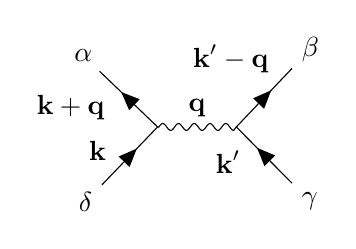
\begin{tikzpicture}
		\begin{feynman}
			% Define vertices
			\vertex (a);
			\vertex[below left= 1 cm of a] (i1) {\(\delta\)};
			\vertex[above left =  1 cm of a] (f1) {\(\alpha\)};
			\vertex[right = 1 cm of a] (b);
			\vertex[below right = 1 cm of b] (i2) {\(\gamma\)};
			\vertex[above right= 1 cm of b] (f2) {\(\beta\)};
			
			% Draw fermion lines
			\diagram*[horizontal'= (a) to (b)] {
				(i1) -- [fermion, edge label=$\textbf{k}$, near start] (a) -- [fermion, edge label=$ \textbf{k} + \textbf{q}$, near end] (f1),
				(i2) -- [fermion, edge label=$\textbf{k}'$, near end] (b) -- [fermion, edge label={$\textbf{k}'- \textbf{q}$}, near end] (f2),
				(a) -- [photon, edge label=$\textbf{q}$] (b),
			};
		\end{feynman}
	\end{tikzpicture}
\end{equation}
$$= \int \frac{d^3 r}{V} \int \frac{d^3 r'}{V} e^{-i \textbf{q}(\textbf{r}-\textbf{r}')} u^*_{\alpha\textbf{k}+\textbf{q}}(\textbf{r})u^*_{\beta\textbf{k}-\textbf{q}}(\textbf{r}') V_{ee} u_{\gamma \textbf{k}'}(\textbf{r}')u_{\delta \textbf{k}}(\textbf{r}),$$
\quad With the 3-D Coulomb interaction have the form:
\begin{equation}
	V_{ee}(\textbf{r}) = \frac{e^2}{\varepsilon |\textbf{r}|}
\end{equation}
\quad Using Fourier transform for the potential, apply long-wave approximation and take the limit \(z \to 0\) to have the 2-D Coulomb matrix elements:
\begin{equation}	V^{\alpha\beta\gamma\delta}_{\textbf{k},\textbf{k}',\textbf{q}} = \frac{e^2}{2\varepsilon L^2} \frac{1}{|\textbf{q}_{\|}|} \braket{u_{\alpha\textbf{k}+\textbf{q}}}{u_{\delta\textbf{k}}}\braket{u_{\beta\textbf{k}'-\textbf{q}}}{u_{\gamma\textbf{k}'}}
\end{equation}
\end{frame}
%\begin{frame}
%	From the equations of motion (in Heisenberg's picture) for \(c^{\dagger}_{\textbf{k}} c_{\textbf{k}}\), we have the equations of motion for the expected value \(\ev{c^{\dagger}_{\textbf{k}} c_{\textbf{k}}}\):
%	\begin{align}
%		\dv{\ev{c^{\dagger}_{\textbf{k}} c_{\textbf{k}}}}{t} =& -\frac{i}{\hbar}\ev{\bigg[H^0 + H^{Coul.} + H_{e-L},c^{\dagger}_{\textbf{k}} c_{\textbf{k}}\bigg]}\nonumber\\
%		=& \frac{i}{\hbar}(\varepsilon_{\lambda}(\textbf{k}) - \varepsilon_{\lambda'}(\textbf{k})) \ev{c^{\dagger}_{\textbf{k}} c_{\textbf{k}}}\nonumber\\
%		\label{Motions}
%		&+ \frac{i}{\hbar} \sum_{\textbf{k}'\textbf{q}} \sum_{\alpha\beta\gamma} V^{\alpha\beta\gamma\lambda}_{\textbf{k},\textbf{k}',\textbf{q}} \ev{c^{\dagger}_{\alpha \textbf{k}+\textbf{q}} c^{\dagger}_{\beta\textbf{k}' - \textbf{q}} c_{\gamma \textbf{k}'}c_{\lambda' \textbf{k}}}\\
%		&+\frac{i}{\hbar} \sum_{\textbf{k}'\textbf{q}} \sum_{\alpha\gamma\delta} V^{\alpha\lambda'\gamma\delta}_{\textbf{k},\textbf{k}',\textbf{q}} \ev{c^{\dagger}_{\lambda \textbf{k}+\textbf{q}} c^{\dagger}_{\alpha\textbf{k}' - \textbf{q}} c_{\gamma \textbf{k}'}c_{\delta\textbf{k}}}\nonumber\\
%		&-\frac{ie}{\hbar m}\textbf{A}(t).\sum_{\mu}(\textbf{p}_{\lambda \mu}(\textbf{k})\rho_{\mu \lambda'}(\textbf{k}) - \rho_{\lambda \mu}(\textbf{k})\textbf{p}_{\mu \lambda'}(\textbf{k})) \nonumber
%	\end{align}
%in which
%\begin{equation}
%	\label{p def}
%	\textbf{p}_{\lambda\lambda'}(\textbf{k}) = \frac{m}{\hbar} \bra{u_{\lambda}} \nabla_{\textbf{k}} H^0_{1e}(\textbf{k})\ket{u_{\lambda'\textbf{k}}}
%\end{equation}
%\end{frame}
\begin{frame}
	From the equations of motion (in Heisenberg's picture) for \(c^{\dagger}_{\textbf{k}} c_{\textbf{k}}\), we have the equations of motion for the expected value \(\ev{c^{\dagger}_{\textbf{k}} c_{\textbf{k}}}\):
		\begin{align}
\dv{\ev{c^{\dagger}_{\textbf{k}} c_{\textbf{k}}}}{t} =& -\frac{i}{\hbar}\ev{\bigg[H^0 + H^{Coul.} + H_{e-L},c^{\dagger}_{\textbf{k}} c_{\textbf{k}}\bigg]}\nonumber\\
=& \frac{i}{\hbar}(\varepsilon_{\lambda}(\textbf{k}) - \varepsilon_{\lambda'}(\textbf{k})) \ev{c^{\dagger}_{\textbf{k}} c_{\textbf{k}}} + \ev{\bigg[H_{e-L},c^{\dagger}_{\textbf{k}} c_{\textbf{k}}\bigg]}\nonumber\\
\label{Motions}
&+ \frac{i}{\hbar} \sum_{\textbf{k}'\textbf{q}} \sum_{\alpha\beta\gamma} V^{\alpha\beta\gamma\lambda}_{\textbf{k},\textbf{k}',\textbf{q}} \ev{c^{\dagger}_{\alpha \textbf{k}+\textbf{q}} c^{\dagger}_{\beta\textbf{k}' - \textbf{q}} c_{\gamma \textbf{k}'}c_{\lambda' \textbf{k}}}\\
&+\frac{i}{\hbar} \sum_{\textbf{k}'\textbf{q}} \sum_{\alpha\gamma\delta} V^{\alpha\lambda'\gamma\delta}_{\textbf{k}',\textbf{k} +\textbf{q},\textbf{q}} \ev{c^{\dagger}_{\lambda \textbf{k}} c^{\dagger}_{\alpha\textbf{k}' + \textbf{q}} c_{\gamma \textbf{k}+\textbf{q}}c_{\delta\textbf{k}'}}\nonumber
\end{align}
Approximation the expected value of four-operator by multiplication of two expected value (Hatree-Fock Approximation):
	\begin{align}
		\ev{c^{\dagger}_{\alpha \textbf{k}+\textbf{q}} c^{\dagger}_{\beta\textbf{k}' - \textbf{q}} c_{\gamma \textbf{k}'}c_{\lambda' \textbf{k}}} &\approx-
		\ev{c^{\dagger}_{\alpha \textbf{k} +\textbf{q}}c_{\gamma \textbf{k}'}}\ev{c^{\dagger}_{\beta\textbf{k}'-\textbf{q}}c_{\lambda' \textbf{k}}}\delta_{\textbf{k}+\textbf{q} \textbf{k}'}\nonumber\\\label{HF Approx}
		 \ev{c^{\dagger}_{\lambda \textbf{k}} c^{\dagger}_{\alpha\textbf{k}' + \textbf{q}} c_{\gamma \textbf{k}+\textbf{q}}c_{\delta\textbf{k}'}}&\approx \ev{c^{\dagger}_{\lambda\textbf{k}+\textbf{q}}c_{\delta \textbf{k}'}} \ev{c^{\dagger}_{\alpha \textbf{k}'+\textbf{q}}c_{\gamma \textbf{k}+\textbf{q}}}\delta_{\textbf{k}' \textbf{k}}
	\end{align}
\end{frame}
\begin{frame}
	Substituting \eqref{HF Approx} into \eqref{Motions} and doing some transformations on the light-matter interaction part to have
\begin{align}
\label{SBE no T}
\dv{\ev{c^{\dagger}_{\lambda\textbf{k}} c_{\lambda'\textbf{k}}}}{t} = &\frac{i}{\hbar} (\varepsilon_{\lambda}(\textbf{k}) - \varepsilon_{\lambda'}(\textbf{k}))\ev{c^{\dagger}_{\lambda\textbf{k}} c_{\lambda'\textbf{k}}}\nonumber\\
&-\frac{i}{\hbar} \sum_{\mu}\bigg(\Sigma_{\mu \lambda}(\textbf{k}) \ev{c^{\dagger}_{\mu\textbf{k}} c_{\lambda'\textbf{k}}} - \ev{c^{\dagger}_{\lambda\textbf{k}} c_{\mu\textbf{k}}} \Sigma_{\mu \lambda'}(\textbf{k})\bigg)
\end{align}
in which
\begin{align}
	\Sigma_{\mu\nu} &= \frac{e\textbf{A}(t)}{m}\textbf{p}_{\mu\nu}(\textbf{k}) - \sum_{\alpha\beta\textbf{q}} V^{\alpha \mu \beta \nu}_{\textbf{k},\textbf{k}+\textbf{q},\textbf{q}}\rho_{\alpha \beta}(\textbf{k+q})\\
	\textbf{p}_{\mu \nu} &= \frac{m}{\hbar}\bra{u_{\lambda \textbf{k}}}\nabla_{\textbf{k}}H^0_{1e}(\textbf{k})\ket{u_{\lambda'}\textbf{k}}\\
	H^0_{1e}(\textbf{k}) &= e^{-i\textbf{k}\textbf{r}} H^0_{1e}(\textbf{r})e^{i\textbf{k}\textbf{r}} = e^{-i\textbf{k}\textbf{r}} \bigg(\frac{\textbf{p}^2}{2m} +V_0(\textbf{r})\bigg)e^{i\textbf{k}\textbf{r}}
\end{align}
\end{frame}
\begin{frame}
Equation \eqref{SBE no T} can describe the transition band between valence bands and conduction bands, but lack of relaxation effect.\\\null
\quad For a better realistic picture, we taken into account the correction from the scattering effect:
\begin{equation}
	\bigg(\dv{\rho(\textbf{k})}{t}\bigg|_{scat.}\bigg)_{\lambda\lambda'} \to - \frac{\rho_{\lambda\lambda'}(\textbf{k})}{T_2}(1-\delta_{\lambda\lambda'})
\end{equation}
\quad The parameter \(T_2\) can be choosing to fit with the experiment, or confirms the exist of the exciton in the absorption spectrum.
\end{frame}
\begin{frame}
Finally, we have the semiconductor Bloch equations\footcite{haug_quantum_2009}:
\begin{align}
	\dv{\rho_{\lambda\lambda'}(\textbf{k})}{t} = &\frac{i}{\hbar} (\varepsilon_{\lambda}(\textbf{k}) - \varepsilon_{\lambda'}(\textbf{k}))\rho_{\lambda\lambda'}(\textbf{k})\nonumber\\
	&-\frac{i}{\hbar} \sum_{\mu}\bigg(\Sigma_{\mu \lambda}(\textbf{k}) \ev{c^{\dagger}_{\mu\textbf{k}} c_{\lambda'\textbf{k}}} - \ev{c^{\dagger}_{\lambda\textbf{k}} c_{\mu\textbf{k}}} \Sigma_{\mu \lambda'}(\textbf{k})\bigg)\\ &-\frac{\rho_{\lambda\lambda'}(\textbf{k})}{T_2}(1-\delta_{\lambda\lambda'}),\nonumber
\end{align}
where,
\begin{equation}
	\Sigma_{\mu\nu} = \frac{e\textbf{A}(t)}{m}\textbf{p}_{\mu\nu}(\textbf{k}) - \sum_{\alpha\beta\textbf{q}} V^{\alpha \mu \beta \nu}_{\textbf{k},\textbf{k}+\textbf{q},\textbf{q}}\rho_{\alpha \beta}(\textbf{k+q})
\end{equation}
\end{frame}
%\subsection{Inter-band Polarization}
\begin{frame}
	\begin{multicols}{2}
		Dipole matrix elements can be obtained through:
		\begin{align}
			&\vec{\xi}_{\mu\nu}(\textbf{k}) = \frac{-i\hbar}{m}\frac{\textbf{p}_{\mu\nu}(\textbf{k})}{\varepsilon_{\mu}(\textbf{k}) - \varepsilon_{\nu}(\textbf{k})}.\\
			&\text{for } \mu \neq \nu \nonumber
		\end{align}
		Time-dependent interband polarization density:
		\begin{align}
			\textbf{P}(t) = &\frac{e}{L^2} \sum_{\textbf{k}} \Tr\bigg[\vec{\xi}(\textbf{k})\rho(\textbf{k},t)\bigg]
		\end{align}
		\columnbreak
		\begin{figure}
			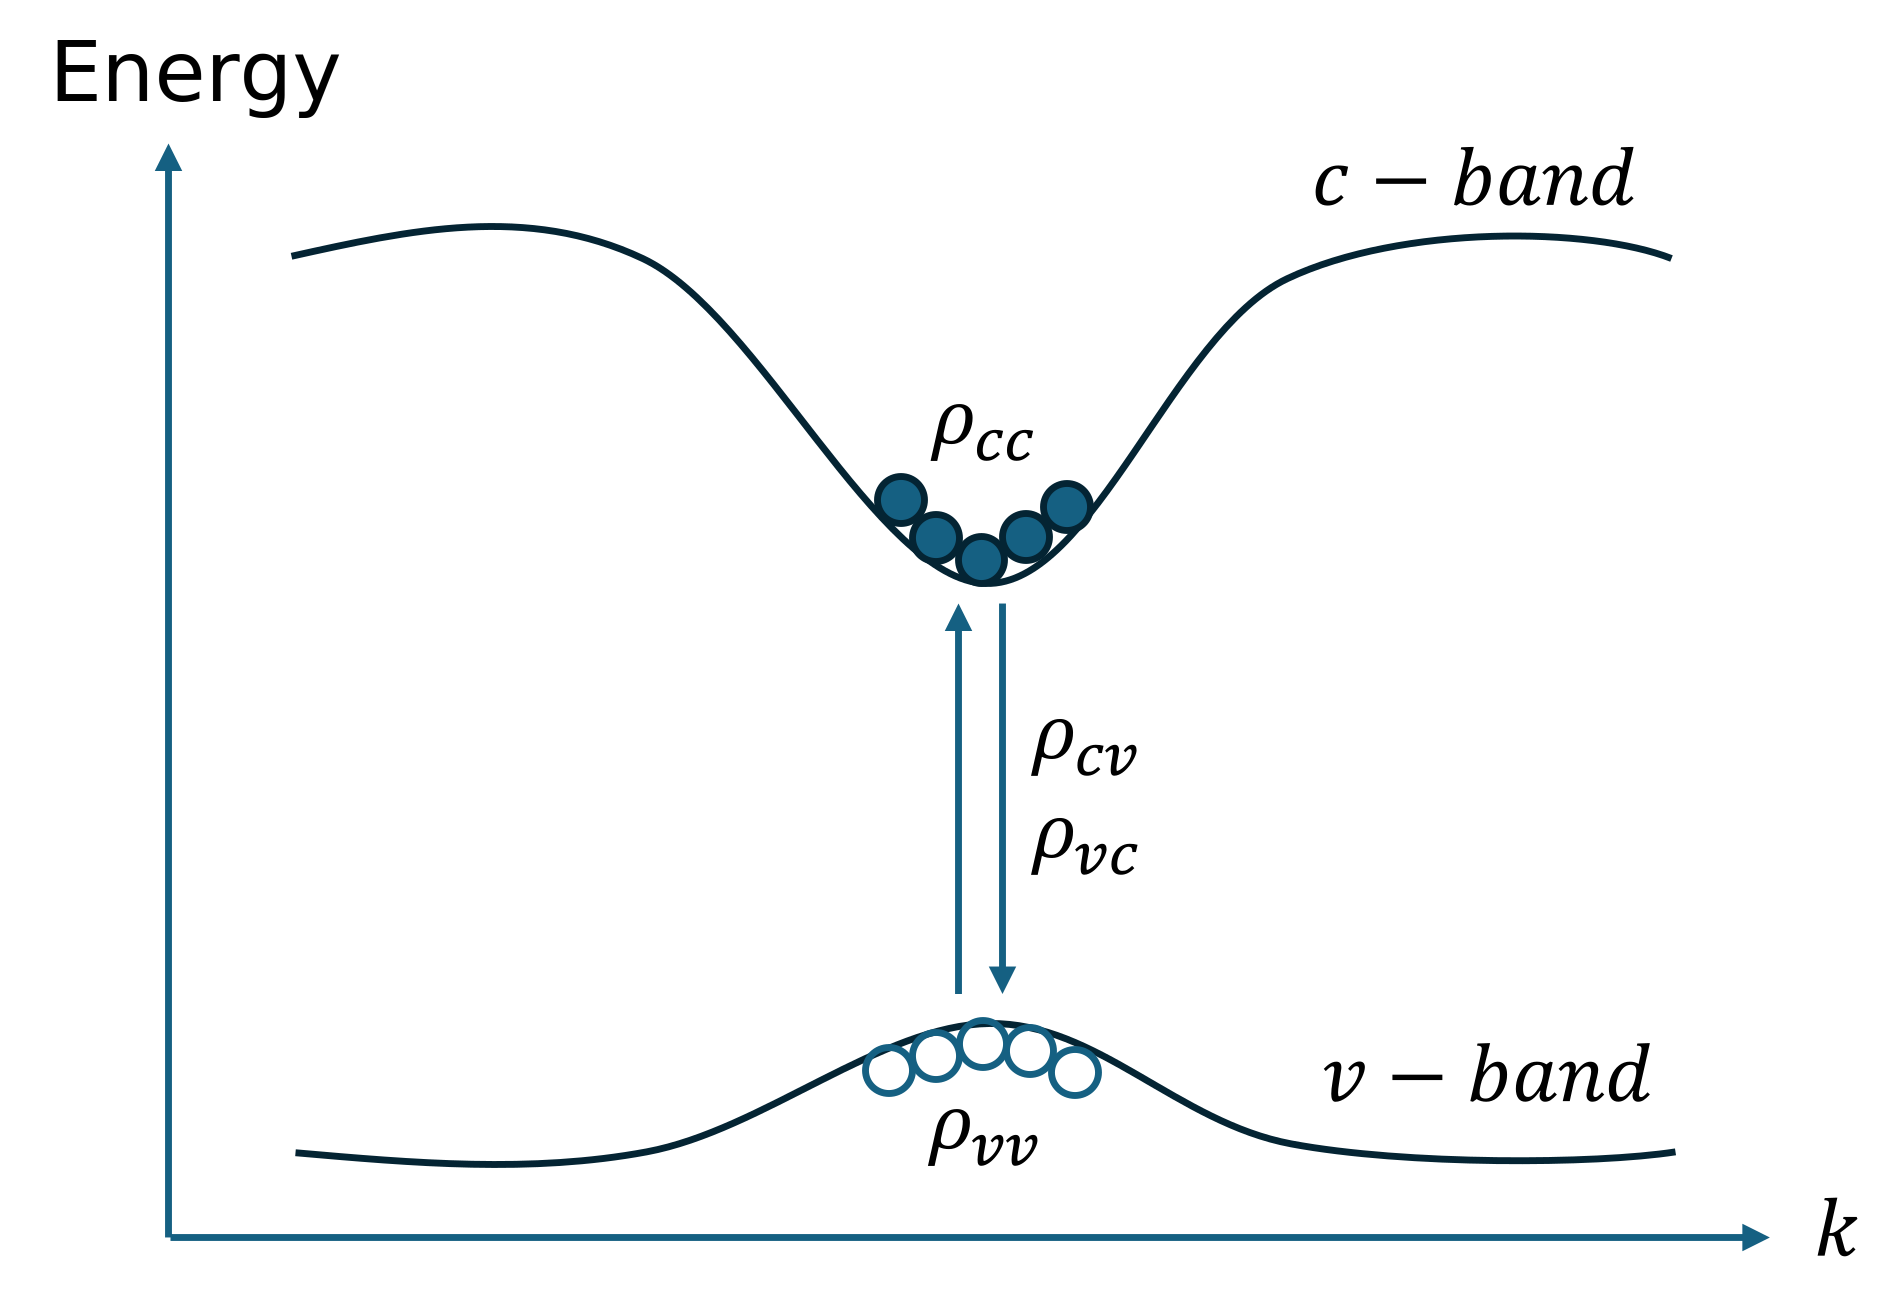
\includegraphics[width=1\linewidth]{images/cvbeamer.pdf}
			\caption{Density matrix element illustration}
		\end{figure}
	\end{multicols}
\end{frame}
\begin{frame}{Three-band Tightbinding model}
	Use basic functions of d-type orbitals: $$\ket{\phi_1} = d_{z^2}, \ket{\phi_2} = d_{xy}, \ket{\phi_3} = d_{x^2- y^2}.$$\\Three-band TB Hamiltonian with SOC has the form:
	\begin{equation*}
		H^{TB}_{6\times 6}(\textbf{k}) = \begin{bmatrix}
			H^{TB}_{3\times 3}(\textbf{k}) + \gamma L_z & 0\\ 0& H^{TB}_{3\times 3}(\textbf{k}) - \gamma L_z
		\end{bmatrix}, \quad L_z= \begin{bmatrix}
			0 & 0 & 0\\
			0 & 0 & i\\
			0 & -i& 0
		\end{bmatrix}.
	\end{equation*}
	\note{The model we use in this work is called the three-band tight-binding models, It using basic function of 3 d-type orbitals as shown. The full Hamiltonian at a k-point is a 6 by 6 matrix when take spin orbit coupling into account.}
\end{frame}
\section{Numerical Results}
\begin{frame}{Numerical Evaluation of The Sum Over k-space}
	\begin{figure}
		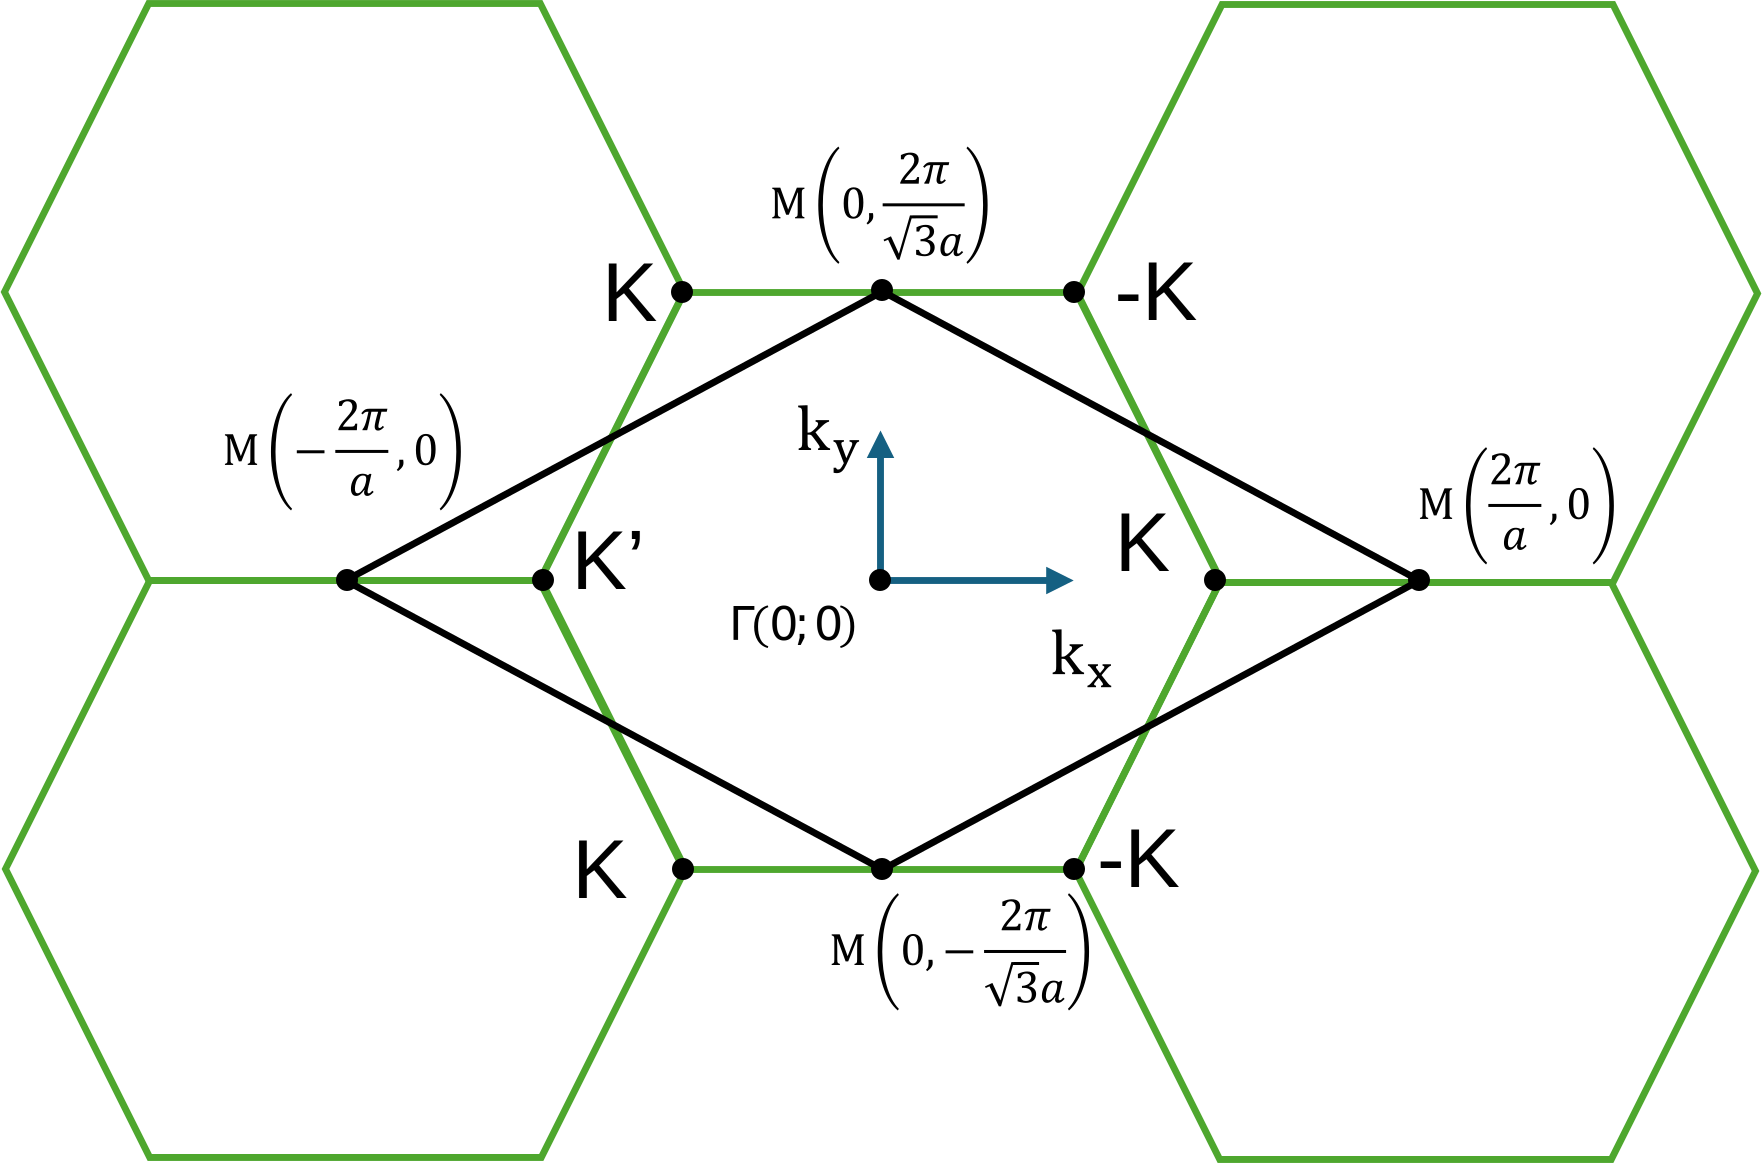
\includegraphics[width=0.5\linewidth]{images/Rhombus.pdf}
		\caption{Rhombus primitive cell}
	\end{figure}
	\begin{equation}
		\sum_{\textbf{k}} ... \to \frac{L^2}{4\pi^2} \int \int_{BZ} dk_x dk_y...
	\end{equation}
	\note[item]{As I have mentioned above, The first Brillouin Zone of monolayer TMD have the shape of Hexagon. However, the hexagon is inconvenient for us when sampling the k-grid, so we will use the rhombus primitive cell with the same area as the hexagon.}
	\note[item]{In order to evaluate the numerical results in the entire BZ, we approximate the sum by this integral.}
\end{frame}
	\begin{frame}{k-Cutoff}
	\begin{figure}
		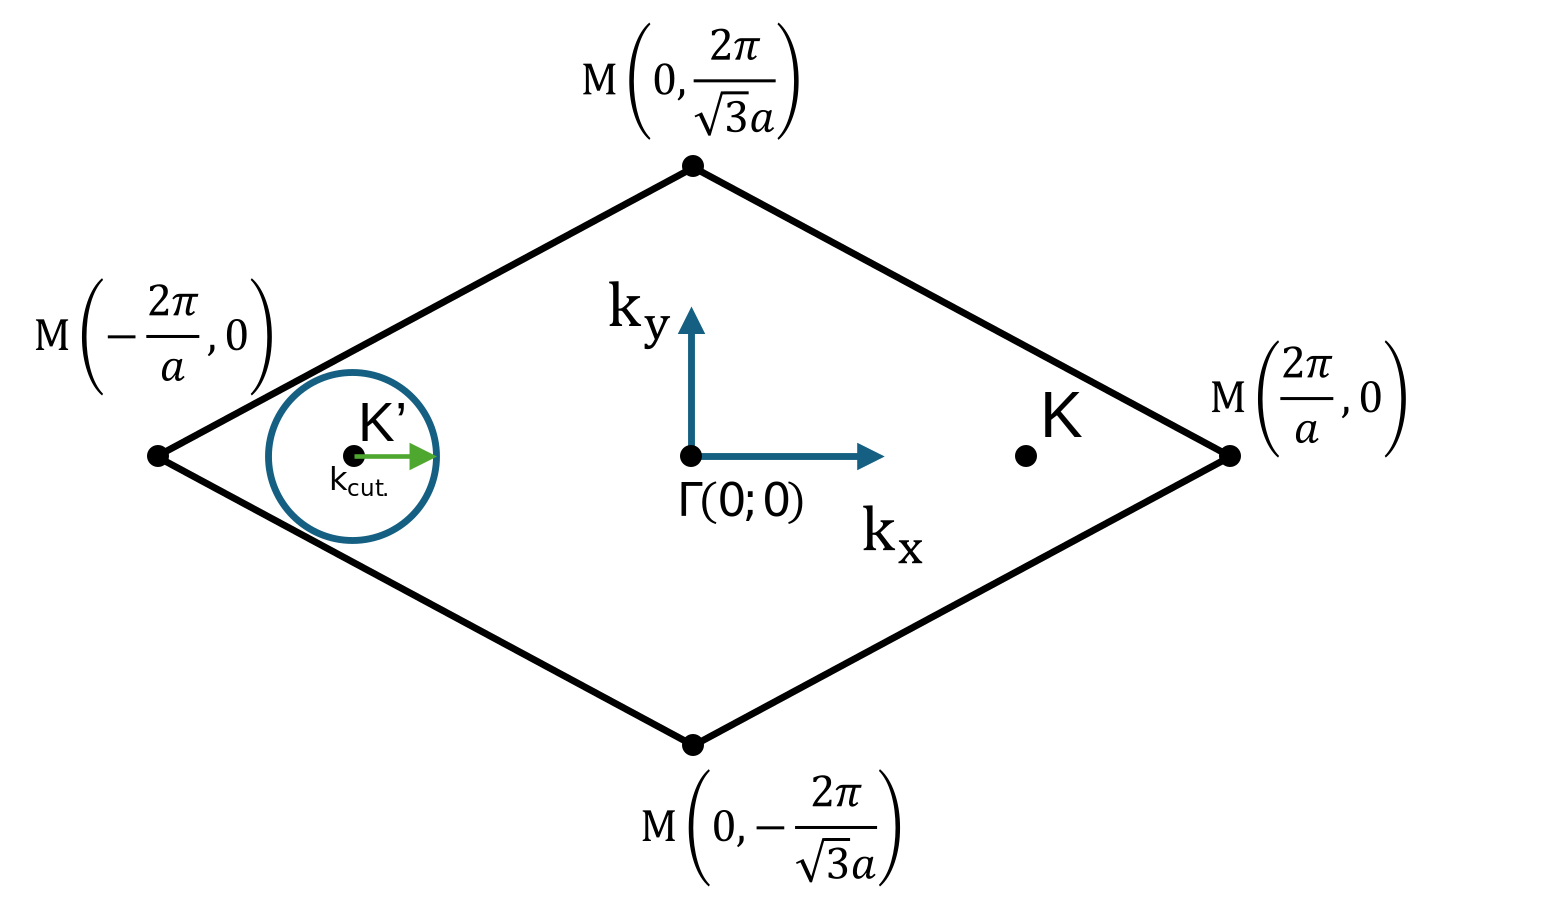
\includegraphics[width=0.75\linewidth]{images/kcutoff.pdf}
	\end{figure}
	For k-points around \textbf{K}' point
	\begin{equation}
		W^{\alpha \mu \beta \nu}_{\textbf{k},\textbf{k}',\textbf{q}} \approx W^{\alpha \mu \beta \nu}_{\textbf{k},\textbf{k}',\textbf{q}} \theta(k_{cut.} - |\textbf{k} - \textbf{k}_{K'}|) \theta(k_{cut.} - |\textbf{k}' - \textbf{k}_{K'}|).
	\end{equation}
	The same for k-points around \textbf{K} point
	\note[item]{When considering the Coulomb interaction, it's essential to account for every k-point in the Rhombus primitive cell. However, including every k-point may result in an overwhelming workload for achieving convergence. For this reason, we employ a technique that focuses specifically on k-points around K and K'.}
	\note[item]{For instance, with the K' point, we draw a circle and calculate the Coulomb interaction only if both points fall within this circle. The same process applies to the K point.}
\end{frame}
\begin{frame}{Electromagnetic Field}
	\begin{multicols}{2}
		The electric field has a Gaussian envelope form:
		\begin{equation}
			\textbf{E}(t) = \textbf{E}_0 \cos(\omega_0 t)e^{-\frac{t^2}{\tau_L^2}}
		\end{equation}
		\begin{itemize}
			\item small $E_0: \rho_{cc}(\textbf{k}) \to 0$
			\item $\hbar \omega_0 = E_{gap.}$
			\item small $\tau_L \to $ rounder Fourier transform's peak around $\omega_0$
		\end{itemize}
		\columnbreak
		\includegraphics[width=1\linewidth]{images/Eat.pdf}
		Absorption coefficient\footcite{haug_quantum_2009}:
		\begin{equation}
			\alpha(\omega) \propto \frac{P(\omega)}{E(\omega)}.
		\end{equation}
	\end{multicols}
	\note[item]{The polarized external field has a Gaussian envelope form with these properties to obtain the weak excitation limit for the linear absorption calculation.}
	\note[item]{The absorption coefficient will be obtained by Eq. (13)}
	\note[item]{P and E is Fourier transformation of polarization density and external field, respectively}
\end{frame}
\begin{frame}
	Experiment measure:
	\begin{multicols}{2}
		\begin{figure}
			\includegraphics[width = 1\linewidth]{images/Experiment.pdf}
			\caption{Measured Absorption Spectrum of $\mathrm{MoS}_2$ at $T=5K$  extracted from Ref.  \footcite{zhang_absorption_2014}} $E_{gap} = 2.15 \pm 0.06$ \(eV\)
		\end{figure}
		Binding energy: \\
		$E_{bind.} = E_{gap} - E_{A} = 0.22$ \(eV\)
		\columnbreak\\
From this figure, we see
		\begin{itemize}
			\item Two resonance labeled by A ($1.93$ \(eV\)) and B ($2.1$ \(eV\)) are exciton peaks (band split due to SOC)
			\item Weak trion peak near A labeled by A' ($18$ \(meV\))
		\end{itemize}
		To fit with experiment, we can change:
		\begin{itemize}
			\item Relative permittivity $\varepsilon$
			\item Dephasing time $T_2$
		\end{itemize}
	\end{multicols}
	\note[item]{The experiment measurement gives us two peaks, labeled as A ($1.93$ \(eV\)) and B ($2.1$ \(eV\)), the binding energy will be obtain by extract the exciton peak from the bandgap energy}
	\note[item]{they also have a weak trion peak in here.}
	\note[item]{To fit with the measurement, we will investigate the relationship between relative permittivity and dephasing time T2 with linear absorption spectrum.}
\end{frame}
\begin{frame}
	\begin{figure}
		\includegraphics[width=0.8\linewidth]{images/varyT2.pdf}
	\end{figure}
Choosing the $T_2$ for clearer Exciton peak:
	\begin{itemize}
		\item The bigger $T_2$, the clearer main Exciton peaks $\to $ confirm two peak.
		\item At $T_2 = 30$ \(fs\) show other smaller peaks $\to $ predict other peaks.
		\note[item]{As we vary T2, two peaks become clearer at bigger T2, which agrees with the measurement.}
		\note[item]{We can also see smaller peaks, which are other exciton peaks but too small to appear in the measurement.}
	\end{itemize}
\end{frame}
\begin{frame}
	\begin{center}		
		\includegraphics[width=0.8\linewidth]{images/varyepsilon.pdf}
	\end{center}
	\begin{itemize}
		\item Choosing the $\varepsilon$ for fitting with the experiment.
		\item For 3-band TB model: $\varepsilon \in (1.5,2.5)$ is in good agreement with measurement binding energy of $E_{bind.}= 0.2-0.5 eV$ \footcite{zhang_absorption_2014}
	\end{itemize}
	\note[item]{The binding energy is affected through the relative permittivity, as we increase the epsilon, two peaks move to the right of the spectrum.}
	\note[item]{With the same epsilon equal to 2.5, we obtain the same results as the experiment, approximately 0.24 eV for the exciton binding energy.}
\end{frame}
%\begin{frame}
%\includegraphics[width=1\linewidth]{images/varynk.pdf}
%\end{frame}
\section{Summary and Outlook}
\begin{frame}
	\begin{block}{Summary:}
		\begin{itemize}
			\item From three-band TB + SBE $\to $ Linear Absorption Spectrum.\\
			\item We confirm the Exciton binding energy in this model is in agreement with experimental data, and predict smaller exciton peaks.
		\end{itemize}
	\end{block}
	\begin{exampleblock}{Further research:}
		\begin{itemize}
			\item High Harmonic Generation
			\item High-order Side-band Generation
			\item Photovoltaic effect
		\end{itemize}
	\end{exampleblock}
	\begin{center}
		Thank you for your listening.
	\end{center}
	\note[item]{So far, we have used the three-band tight-binding model and semiconductor Bloch equations to calculate the linear absorption spectrum. We confirm that this model matches the results with the experiment data and also predicts smaller exciton peaks.}
	\note[item]{For further results, we can include the many-body interaction in calculating other phenomena for a realistic picture of TMD's properties.}
\end{frame}
\begin{frame}
\printbibliography
\end{frame}
\end{document}